\documentclass[titlepage,a4paper]{article}

\usepackage{a4wide}
\usepackage[colorlinks=true,linkcolor=black,urlcolor=blue,bookmarksopen=true]{hyperref}
\usepackage{bookmark}
\usepackage{fancyhdr}
\usepackage[spanish]{babel}
\usepackage[utf8]{inputenc}
\usepackage[T1]{fontenc}
\usepackage{graphicx}
\usepackage{float}

\usepackage{minted} %codigo

\pagestyle{fancy} % Encabezado y pie de página
\fancyhf{}
\fancyhead[L]{TP1 - Grupo 1}
\fancyhead[R]{Análisis Numérico - FIUBA}
\renewcommand{\headrulewidth}{0.4pt}
\fancyfoot[C]{\thepage}
\renewcommand{\footrulewidth}{0.4pt}
\usepackage[utf8]{inputenc}


\begin{document}
\begin{titlepage} % Carátula
	\hfill
\includegraphics[width=6cm]{logofiuba.jpg}
    \centering
    \vfill
    \Huge \textbf{Trabajo Práctico 1}
    \vskip2cm
    \Large [ 75.12 - 95.04 ] Análisis Numérico\\
    Curso 5 \\ 
    Primer cuatrimestre de 2020 
    \vfill
    \vfill
    \vfill
\end{titlepage}

\tableofcontents % Índice general

\section{Introducción}\label{sec:intro}
En este trabajo práctico creamos un programa para la búsqueda de raíces de funciones a través de los siguientes métodos numéricos aprendidos en la materia:
\begin{itemize}
\item Bisección
\item Newton-Raphson
\item Newton-Raphson modificado
\item Secante
\end{itemize}
\\Con este fin graficamos las funciones, utilizando la biblioteca matplotlib.pyplot para conocer el intervalo en el cuál se encuentra la raíz, teniendo de esa manera las semillas necesarias para los métodos. Obtenidas las raíces, con la historia de los resultados, pasamos a analizar los distintos metodos viendo los ordenes de convergencia y su conveniencia en tiempos de cómputo y error en el resultado.
Luego, para verificar los resultados, calculamos las raíces mediante la biblioteca de Python numpy, de esta manera pudimos ver el correcto funcionamiento de las funciones programadas.

\section{Objetivos}\label{sec:objetivos}
El objetivo del trabajo práctico es obtener la raíz de las tres funciones dadas mediante los métodos numéricos indicados, luego, analizar el orden de convergencia P y la constante asintótica \begin{align}
\lambda
\end{align}. 

\section{Gráficos}\label{sec:graficos}

\begin{figure}[H]
\centering
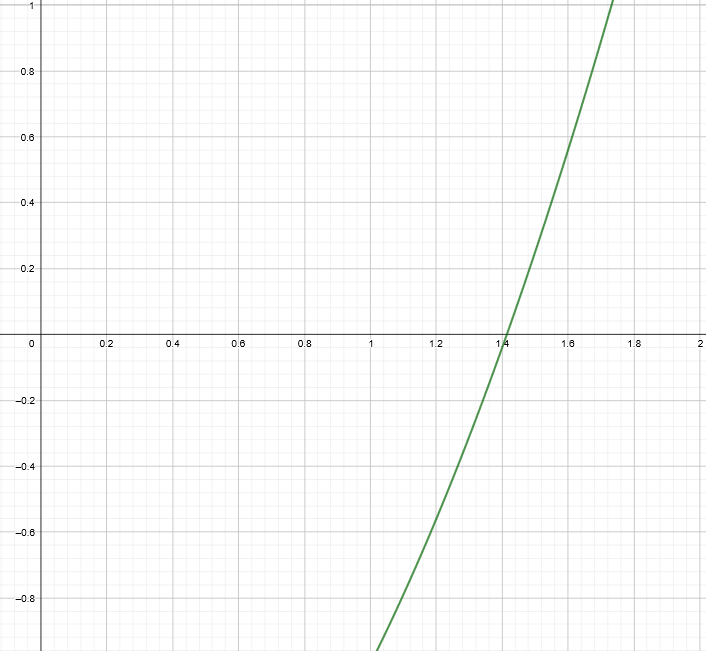
\includegraphics[width=0.8\textwidth]{funcion1.png}
\caption{\label{fig:class01}Gráfico correspondiente a la primera función en el intervalo [0;2].}
\end{figure}

\begin{figure}[H]
\centering
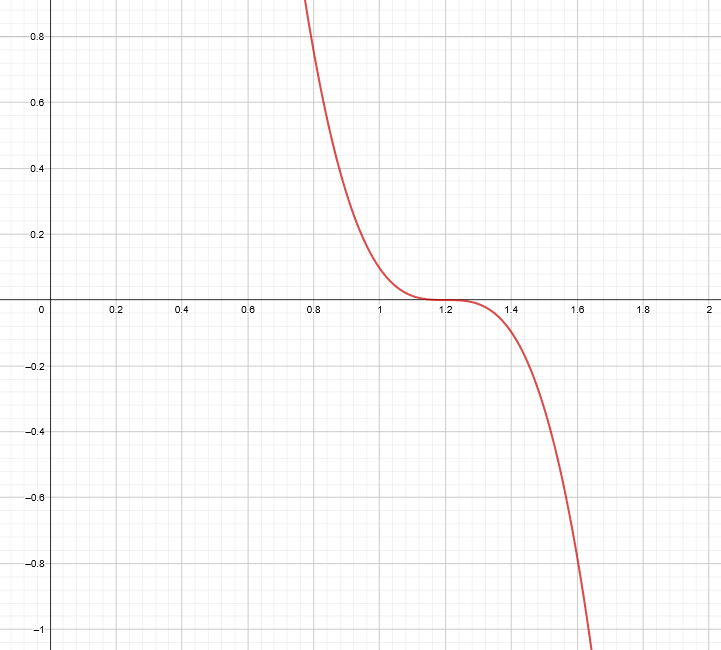
\includegraphics[width=0.8\textwidth]{funcion2.png}
\caption{\label{fig:class01}Gráfico correspondiente a la segunda función en el intervalo [0;2].}
\end{figure}

\begin{figure}[H]
\centering
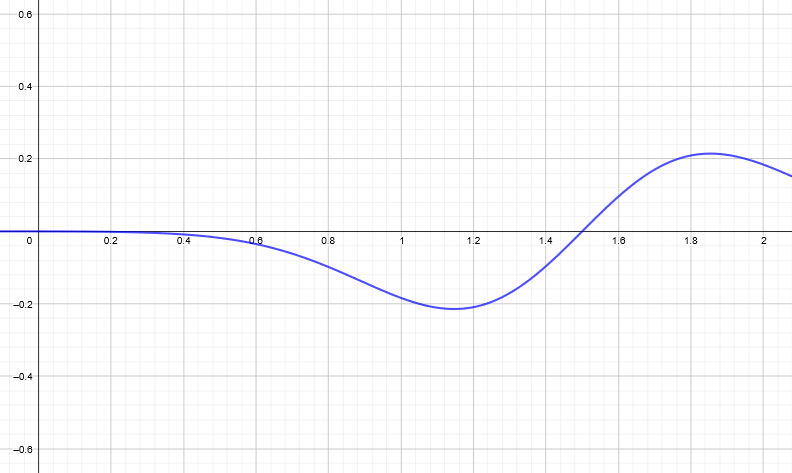
\includegraphics[width=0.8\textwidth]{funcion3.png}
\caption{\label{fig:class01}Gráfico correspondiente a la tercera función en el intervalo [0;2].}
\end{figure}

\section{Búsqueda de raíces}\label{sec:busqueda_raices}

\subsection{Bisección}\label{sec:biseccion}
El método de bisección halla la raíz utilizada mediante la siguiente fórmula por métodos iterativos hasta que \begin{align}
f(r_n)=0\pm \mbox{cota de error}
\end{align} , tomando los límites iniciales de intervalo \begin{align}
{a_n}
\end{align} y 
\begin{align}
{b_n}
\end{align}:
\\\begin{align}
{{\mbox{Sea }r_n = \frac{a_n+b_n}{2}\mbox{, entonces, en la siguiente iteración}\\\end{align}
\begin{align}\centering
\quad a_{n+1} =\left\{ \begin{array}{lcc}
             a_n & \mbox{si } f(a_n)\cdot f(r_n) <0 \\
             \\ r_n & \mbox{si } f(a_n)\cdot f(r_n) > 0 \\
             \end{array}
   \right. \end{align}
\\
\begin{align}\centering
\quad b_{n+1} =\left\{ \begin{array}{lcc}
             b_n & \mbox{ si } f(b_n)\cdot f(r_n) < 0 \\
             \\r_n & \mbox{ si } f(b_n)\cdot f(r_n) > 0 \\
             \end{array}
   \right. }
}}\end{align}
\\\\Los resultados obtenidos fueron los siguientes:


\subsection{Newton-Raphson}\label{sec:biseccion}
El método de Newton-Raphson halla la raíz a partir de una semilla inicial, iterando la siguiente sucesión
\begin{align}\centering
\quad r_{n} =r_{n-1}-\frac{f (r_{n-1})}{f'(r_{n-1})}
}}\end{align} hasta que \begin{align}
r_{n}-r_{n-1} < \mbox{cota de error}
\end{align}
\\\\Los resultados obtenidos fueron los siguientes:


\subsection{Newton-Raphson modificado}\label{sec:biseccion}
El método de Newton-Raphson modificado le aplica el método de Newton-Raphson a la función
\begin{align}
\mu =\frac{f (x)}{f'(x)}
}}\end{align} y halla la raíz a partir de una semilla inicial, iterando la siguiente sucesión
\begin{align}\centering
\quad r_{n+1}=r_n-\frac{f(p_n).f'(r_n)} {f'(r_n)^2-f(r_n).f''(r_n)}
}}\end{align} hasta que \begin{align}
r_{n}-r_{n-1} < \mbox{cota de error}
\end{align}
\\\\Los resultados obtenidos fueron los siguientes:

\subsection{Secante}\label{sec:biseccion}
El método de la secante halla la raíz a partir de una semilla inicial, iterando la siguiente sucesión
\begin{align}\centering
\quad r_{n} =r_{n-1}-\frac{f (r_{n-1})*(r_{n-1}-r_{n-2})}{f(r_{n-1})-f(r_{n-2})}
}}\end{align} hasta que \begin{align}
r_{n}-r_{n-1} < \mbox{cota de error}
\end{align}
\\\\Los resultados obtenidos fueron los siguientes:

\section{Comparación de resultados}\label{sec:comparacion_resultados}
Neque porro quisquam est qui dolorem ipsum quia dolor sit amet, consectetur, adipisci velit.

\end{document}
